\documentclass[a4paper,11pt]{article}

\usepackage[T1]{fontenc}
\usepackage[utf8]{inputenc}
\usepackage[czech]{babel}
\usepackage[top=3cm, left=2cm, textwidth=17cm, textheight=24cm]{geometry}
\usepackage{multirow}
\usepackage[ruled, czech, linesnumbered, noline, longend]{algorithm2e}
\usepackage{graphics}
\usepackage{pdflscape}
\usepackage{float}
\usepackage{tabularx}
\usepackage{array}
\usepackage{amsmath}


\usepackage[unicode, hidelinks]{hyperref}
\usepackage[nodayofweek]{datetime}
\usepackage[hyphenbreaks]{breakurl}
\usepackage{csquotes}
\usepackage{graphicx}
 
\begin{document}

\begin{titlepage}
    \begin{center}
        
        \Huge
        \textsc{Vysoké učení technické v~Brně}\\[0.1em]
        
        \huge
        \textsc{Fakulta~informačních technologií}
        
        \vspace*{\stretch{0.382}}
        
        \LARGE
        Modelování a simulace \\
        Elektromobilita v Brně

        \vspace*{\stretch{0.618}}
    \end{center}
    
    {\large \today \hfill Tomáš Dolák (xdolak09), Monika Záhradníková (xzahra33)}
\end{titlepage}

\newpage
\tableofcontents

\newpage
\label{firstpage}

\section{Úvod}
Jako téma našeho projektu jsme si zvolili modelování elektromobility v Brně. Elektromobilita je aktuálním trendem,
který se v posledních letech stává stále populárnějším a je pravděpodobné, že tomu bude tak i nadále.
V rámci projektu se zaměříme na modelování elektromobily v Brně s cílem určit, zda je Brno připraveno
na budoucnost.\cite{simlib_cpp}

\section{Autoři simulace}
Autoři této simulační studie do předmětu IMS (Modelování a simulace) jsou:

\begin{itemize}
    \item Tomáš Dolák, \href{mailto:xdolak09@stud.fit.vutbr.cz}{\texttt{xdolak09@stud.fit.vutbr.cz}}
    \item Monika Záhradníková, \href{mailto:xzahra33@stud.fit.vutbr.cz}{\texttt{xzahra33@stud.fit.vutbr.cz}} \\
\end{itemize}

\section{Cíle projektu}
Cílem projektu bylo vytvořit model, který bude schopen simulovat chování nabíjení elektromobilů 
v Brně. Model zahrnuje informace o elektromobilech a nabíjecích stanicích vyskytující se
v Brně. Doménou modelu bude schopenost simulovat zátěž sítě nabíjecích stanic na základě zájmu o využítí 
stanic, celkové struktuře této sítě a to v závislosti na části dne. Chování modelu, lze ovlivnit
jeho parametry volání, mezi které patří počet elektromobilů nacházející se ve městě, kolik 
procent z nich využíva veřejné stanice denně, počet stanic (lze specifikovat více druhů viz. 
kapitola~\ref{sec:stanice}), a dále čas kdy simulace bude probíhat - celý den, tedy 24 hodin, denní režim a noční
režim. Tento model lze využít k analýze a optimalizaci stavu sítě stanic pro nabíjení elektrických
vozidel v Brně.

\section{Validita modelu}
Model byl otestován s aktuálním stavem sítě a zájmem o nabíjení na veřejných stanicicích a pomocí 
experimentů, kde bylo zkoumáno, aktuální složení sítě a odhadovaným množstvím elektromobilů v Brně
v roce 2030. K realizaci modulu byly využity jak veřejná data - viz. \ref{sec:zdroje} neveřejná data, 
konkrétní data ani zdroje nemohou být publikovány. Tyto informace byly použity k vytvoření představy 
o aktuálním stavu elektromobily v Brně a k ověření správnosti modelu. 

\section{Rozbor tématu a použitých metod/technologií}
Pro korektní modelování elektromobility je potřeba si nejprve uvědomit, jak elektromobily fungují, 
jaké jsou jejich vlastnosti/parametry, jelikož, elektrická vozidla budou v modelu představovat transakce.
Je třeba si také uvědomit typy a počty nabíjecích stanic v Brně, tedy strukturu sítě, jak probíhá
nabíjecí cyklus, jaké jsou fáze tohoto cyklus (tzv. SoC -- State of Charge) a v neposlední řadě 
jaká je vůbec poptávka po nabíjecích stanicích.  

\subsection{Elektrické vozidlo}
Tedy naše tranksakce, mezi hlavní aspekty, ovlivňující chování elektromobilu, patří v prvé řadě 
jeho motor, akumulátor/baterie a jeho vnitřní nabíječka, jež je využita v případě nabíjení pomocí
střídavého proudu.

\subsubsection{Elektromotor}
U každého vozidla je nejdůležitější jeho pohon a palivo. Pro elektromobily je pohon zajištěn 
elektromotorem, který je základní součástí elektrického hnacího systému. Elektromotor přeměňuje 
elektrickou energii z baterie na mechanickou energii potřebnou pro pohyb vozidla a skládá se 
primárně ze dvou hlavních částí -- rotoru a statoru. \cite{typy_elektromotoru}

Rotor je pohyblivá část elektromotoru. Jedná se o součást, která se otáčí a přenáší mechanickou 
energii na hnací ústrojí vozidla. Pohyb rotoru je vyvolán magnetickými silami, které vznikají mezi 
ním a statorem. Rotor může být vyroben z permanentních magnetů (v motorech s permanentními magnety) 
nebo z vodivých materiálů, které reagují na elektromagnetické pole statoru (v asynchronních motorech). \cite{elektromotor}

Stator je naopak pevná část elektromotoru, která obklopuje rotor. Obsahuje sady cívek, které jsou 
napájeny elektrickým proudem z baterie. Když těmito cívkami prochází proud, vytváří elektromagnetické 
pole. Toto pole interaguje s magnetickým polem rotoru a vytváří točivý moment, který pohání rotor. \cite{elektromotor}

\begin{figure}[H]
    \centering
    \scalebox{0.25}{
        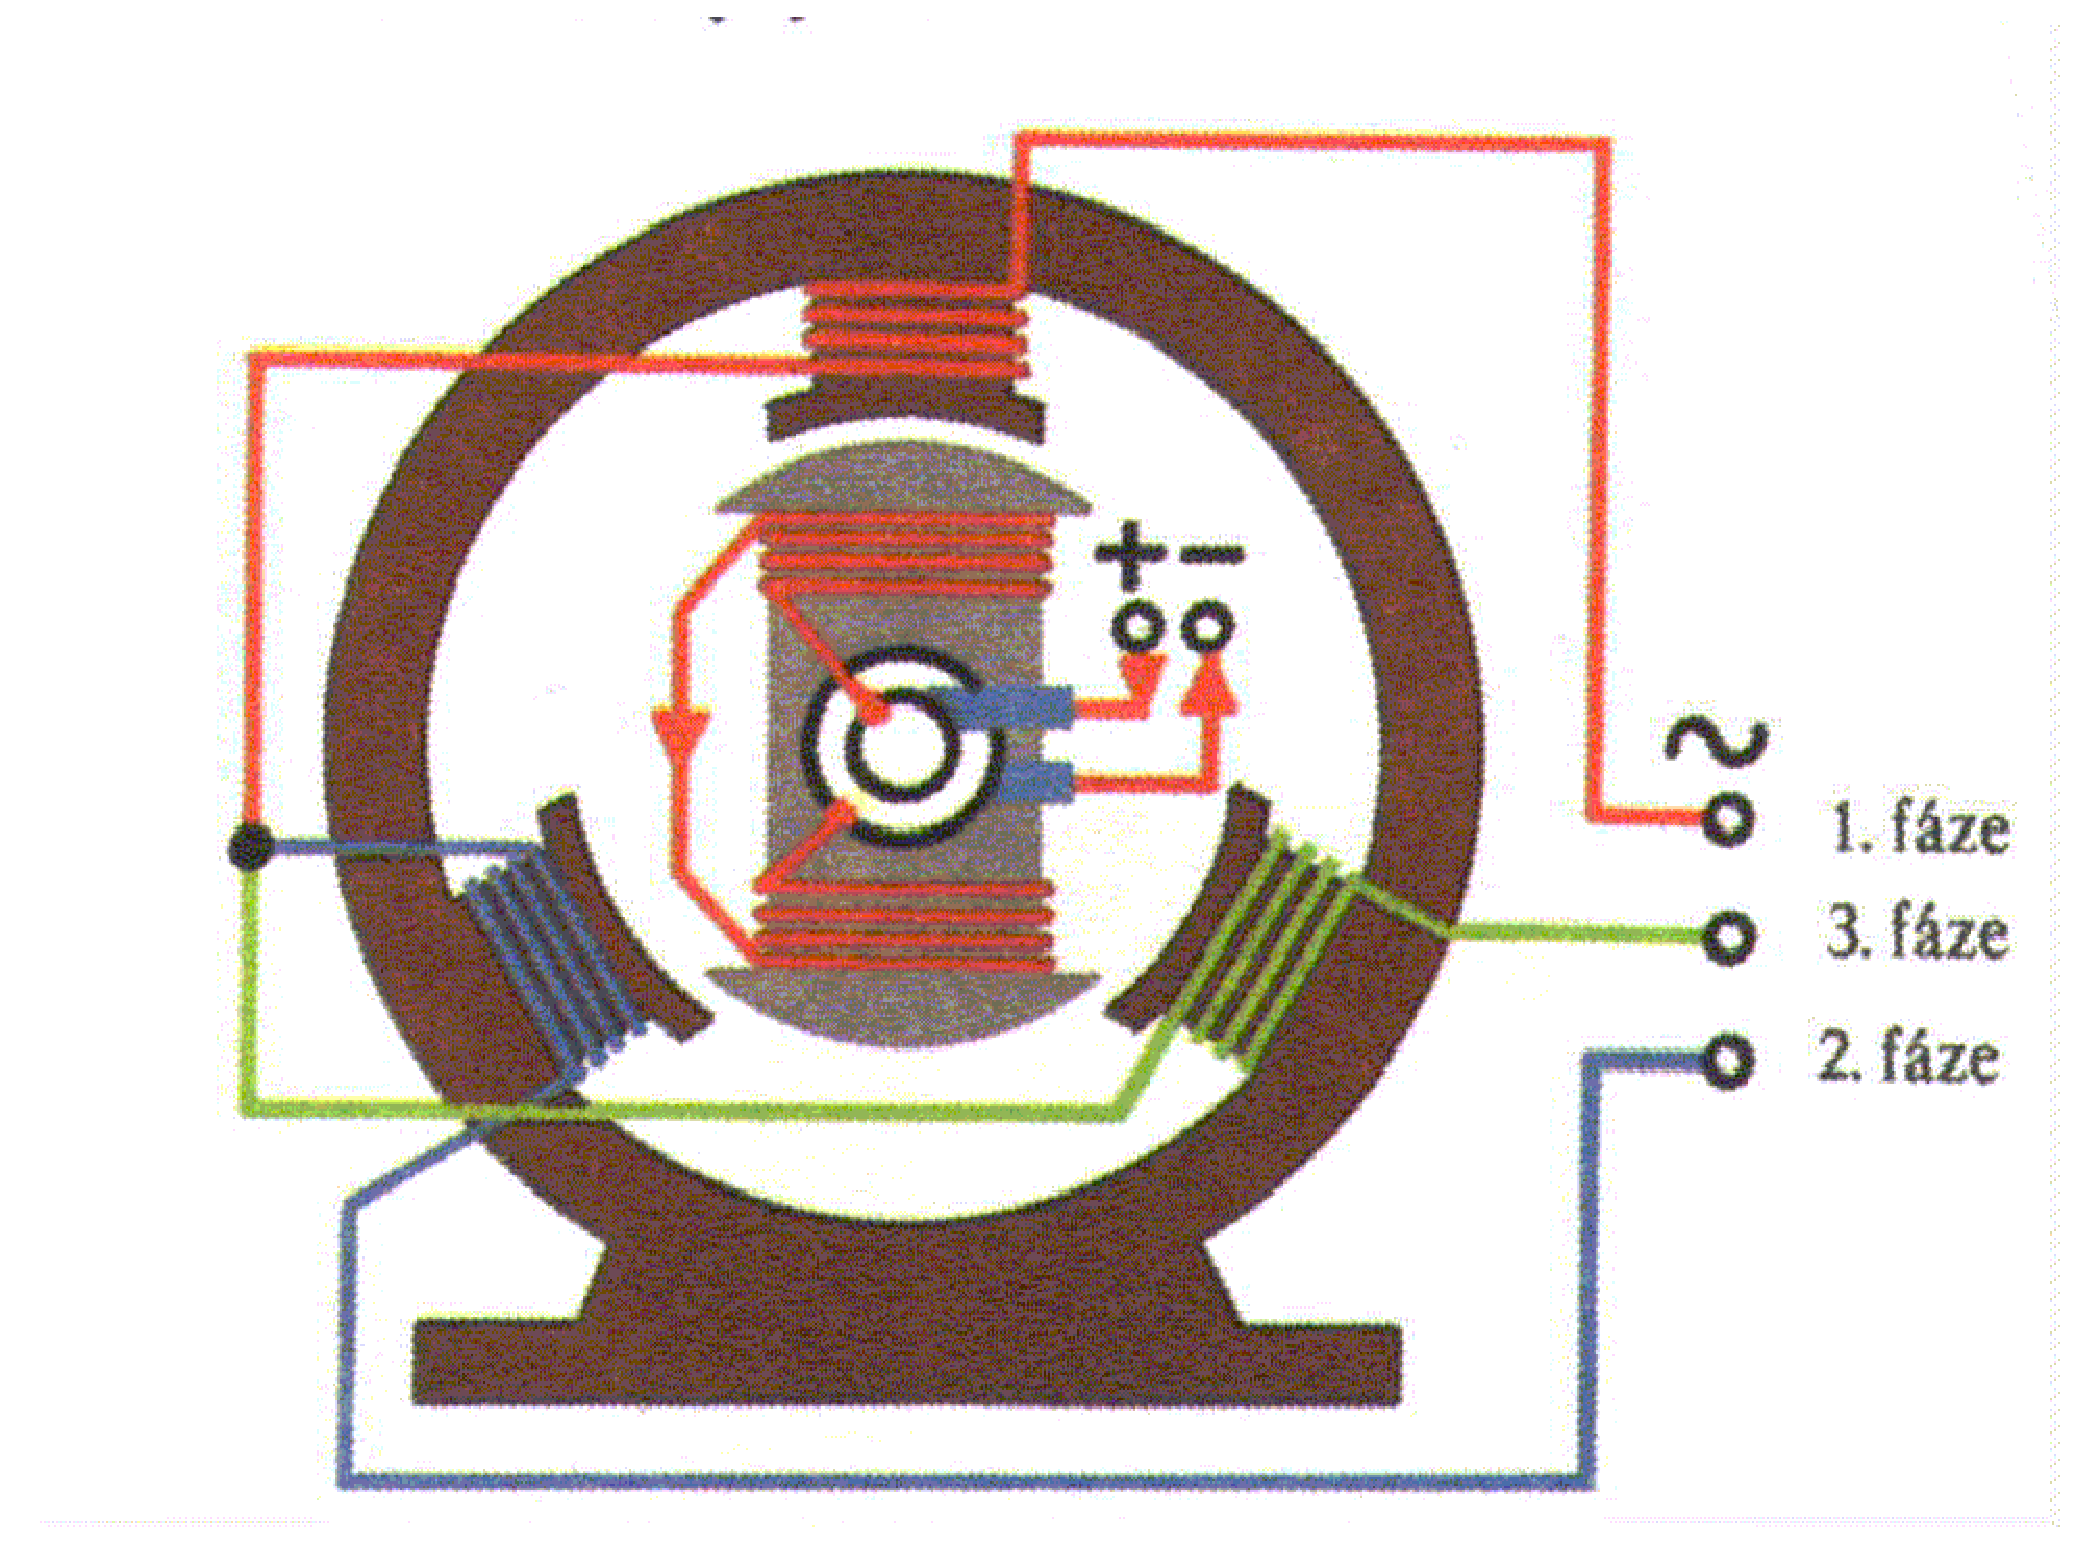
\includegraphics{synchroni-elektromotor.eps}
    }
    \caption{Schéma synchronního elektromotoru \cite{elektromotor}}
    \label{figure:synchroni-elektromotor}
\end{figure}

\subsubsection{Baterie}

\label{batteries}
Baterie je další důležitou součástí elektromobilu. Stejně jako existuje více typů elektromotorů, 
liší se i baterie, používané jednotlivými výrobci. V zásadě se ale jedná o lithium-iontové baterie
(varianty LIB a Li-NMC), poskytující přijatelný poměr mezi kapacitou, hmotností a prostorem, který 
zabírají.\cite{baterie_ev_wiki} Liší se však v použitelné kapacitě této baterie, které se pohybuje 
v rozmezí od 123 kWh, po 21.3 kWh na základě dat z webové stránky www.ev-database.org \cite{ev_database}, 
poskytující databázi o elektromobilech. Tato databáze zároveň poskytuje informaci o průměrné kapacitě
baterie, která činí 71.6 kWh, tato hodnota bude dále v modelu využita pro výpočet času stráveného autem
nabíjením na stanici.

Je důležité zmínit, že baterie postupem času degraduje. S rostoucím počtem najetých kilometrů se postupně snižuje její maximální kapacita. Tento proces je přirozenou vlastností lithium-iontových baterií a nelze jej zcela zastavit, lze jej však vhodným způsobem zpomalit. Pro co nejdelší životnost a zdraví baterie je doporučeno udržovat její kapacitu v rozmezí 20–80~\%. To znamená vyvarovat se jak hlubokému vybití, tak i častému nabíjení na 100~\%. Tyto extrémní stavy vedou k urychlenému opotřebení článků. Tuto informaci budeme dále využívat při návrhu modelu a simulace.\cite{battery-health}

\subsubsection{Typy nabíjení}
Elektromobil, lze nabíjet hned několika způsoby, faktorů je mnoho, výkon elektrostanice, typ proudu, 
konektor,... My jsme se v našem modelu rozhodli zachovat pouze podstatné parametry, které v našem 
případě budou mít největší vliv na chování elektromobilů a to nabíjecí výkon a druh proudu. 
Elektromobil, zde obvykle nabíjet jak stejnosměrným proudem, tak střídavým proudem.

\begin{figure}[H]
    \centering
    \scalebox{0.13}{
        \includegraphics{difference-between-ac-and-cd-charging-ev.eps}
    }
    \caption{Rozdíl mezi nabíjením střídavým a stejnosměrným proudem \cite{rozdil_mezi_ac_dc_nabijenim}}
    \label{figure:difference-between-ac-and-cd-charging-ev}
\end{figure}

Rozdíl ale je v jejich efektivitě, u nabíjení střídavým proudem nezáleží pouze na výkonu nabíjecí stanice, 
ale také na samotném vozidle. Baterie elektromobilu je schopna pracovat pouze se stejnosměrným proudem, 
proto je potřeba mít v elektromobilu vestavěný měnič (palubní nabíječka), který střídavý proud převede 
na stejnosměrný. Palubní nabíječka obvykle pracuje s výkonem 3,6 kW, 7,2 kW, 11 kW nebo 22 kW,
který obvykle limituje nabíjení elektromobilu, daleko víc než výkon nabíjecí stanice. \cite{nabijeni_ev}
Zato nabíjení stejnosměrným proudem je mnohem efektivnější, nemusí se měnit typ proud a nabíjení není limitováno
vůbec výkonem palubní nabíječky. Tyto nabíjecí stanice obvykle poskytují výkon 50 kW, 150 kW nebo až 350 kW.\cite{nabijeni_ev, data_brno}

U nabíjení stejnosměrným proudem se standardně cyklus nabíjení skládá ze tří fází (tzv. SoC -- State of Charge), první
fáze se pohybuje v rozmezí 0 až 20\% kapacity baterie, zde pomalu výkon narůstá, tato fáze je omezena komunikací
mezi nabíjecí stanicí a elektromobilem a také teplotou baterie. Druhá fáze začíná na 20\% až 80\% zde se na začátku
stavu dosáhne maximální výkon stanice (většínou stanice jelikož elektromobily mají zpravidla povolený větší maximální výkon
než dnešní stanice standardně nabízejí) a následně začíná pokles, tento sestupný trend nastává jak se baterie plní a
zároveň se přehřívá. Poslední fází je rozsah mezi 80\% až 100\%, zde se výkon nabíjení opět snižuje, jelikož
dochází k protekci před přebitím baterie a i chemický proces, ke kterému dochází v baterii je méně efektivní 
při vyšších úrovních nabití, což má za následek že stejný nabíjecí proud má menší dopad na zvýšení kapacity. \cite{nabijeci_krivka}

\begin{figure}[H]
    \centering
    \scalebox{0.25}{
        \includegraphics{ac-dc-charging-efficency.eps}
    }
    \caption{Efektivita nabíjení pomocí stejnosměrného a střídavého proudu \cite{rozdil_mezi_ac_dc_nabijenim_graf}}
    \label{figure:ac-dc-charging-efficency}
\end{figure}

U nabíjení na střídavý proud je situace jiná, tím, že je výkon primárně limitován elektromobilem -- tedy palubní nabíječkou 
(OBC - On-Board Charger), výrobce automobilu zaručuje, že baterie je schopna pracovat s určitým výkonem, který externí
nabíjecí stanice ve většině případů schopna poskytnout. Typickými limity palubní nabíječky je od 6.6kW do 22kW. \cite{we_power_your_car_obc} 
Z tohoto rozsahu se vycházi i výběr nabíjecích stanic se střídavým proudem v popisovaném modelu, viz. tabulka \ref{table:charging-stations-distribution}.

\subsection{Elektronabíjecí stanice}

\subsubsection{Jak je na tom s elektro stanicemi Brno?}
\label{sec:stanice}
V Brně je celkem 173 veřejných nabíjecích stanic, vyplývající z dat z webu www.data.brno.cz\cite{data_brno},
na této stránce je i vytvořený dataset s mapou, kde jsou všechna data zaznamenána a zpřístupněna veřejnosti.
My jsme tento dataset využili a zpracovaná data, lze najít ve složce \texttt{data/}. V souboru \texttt{charging\_stations\_cez.json}
obsahuje seznam všech veřejných nabíjecích stanic společnosti ČEZ, \texttt{charging\_stations\_PRE.pdf} obsahuje
list stanic skupiny PRE (Pražská energetika), mezi další velké hráče na poli elektromobility v Brně patří společnosti
Teplárny Brno a.s. a E.ON. Dvě 11kW stanice, devětadvacet 22kW stanic, jedenáct 50kW stanic a 5 stanic o výkonu 150kW, 
poskytuje E.ON, jak vyplývá z dat dostupných na webu \href{https://www.eon-drive.cz/mapa/}{www.eon-drive.cz/mapa/}.
Zato společnosti Teplárny Brno a.s. disponuje celkem 132 nabíjecími stanicemi. Z těchto 132 stanic tvoří většínu -- 120 
nabíječky se střídavým proudem o výkonu 22 kW, a zbylých 12 nabíjecích stanic je stejnosměrných s výkonem 150 kW. 
Data společnosti Teplárny Brno a.s byly získány pomocí informací z mapy na stránce 
\href{https://www.emobilitabrno.cz/cs/verejne-dobijecky}{www.emobilitabrno.cz/cs/verejne-dobijecky}.
Soubor \texttt{charging\_stations\_others.xlsx} stanice, které jsou vlastněny menšími firmami.
V zásadě Brno disponuje nabíjecími stanicemi s výkonem od 3.7 kW (AC) až po 108 kW (DC), a nabíjecích bodů je 
celkově 173. \cite{eon_data, emobilita_data}

% TODO: popis jak jsme vyuzili dataset a jak jsme ho zpracovali
\subsubsection{Zpracování datasetu}
\label{dataset-processing}
Data z datasetu poskytnutého portálem www.data.brno.cz \cite{data_brno}, bylo třeba nejprve zpracovat a určit 
aktuální situaci v Brně. Zpracovaný dataset nacházející se v souboru \texttt{brno\_charging\_summary.xlsx},
obsahuje tedy roztřízené elektrostanice podle typu proudu (stejnosměrný/střídavý) a výkonu nabíjení. Jak již bylo
řečeno Brno poskytuje nabíjecí stanice s výkonem od 3.7 kW (AC) až po 108 kW (DC), a nabíjecích bodů je celkově 173,
do úvahy jsme však vybrali pouze stanice s nabíjecím výkonem od 11 kW, jelikož systému s výkonem 3.7 kW se dnes již 
neimplementují do veřejných nabíjecích stanic, jelikož nabíjení by trvalo příliš dlouho -- vznikají tak malé ztráty
modelu, které jsou však tolerovány, takový elektromobil s průměrnou kapacitou baterie 71.6 kWh by se z 0 na 100 procent 
nabíjel 19.43 hodin, model poskytuje simulaci trvající maximálně 24 hodin, tedy za dobu simulace by byl nabito pouze jedno
vozidlo\footnote{V první fázi z 0 do 20 procent za 3.9, v druhé fázi od 20 do 80 procent by to trvalo 11.93 a poslední 
fáze z 80 do 100 procent by opět trvala 3.9 hodiny}.

\begin{table}[h!]
    \centering
    \vspace{0.5cm} % Space before table
    \begin{tabular}{|c|c|c|c|}
        \hline
        \textbf{Stanice} & \textbf{Výkon stanice} & \textbf{Typ stanice} & \textbf{Počet stanic}\\
        \hline
        11kW  AC &  11kW   & střídavý proud       & 6  \\
        \hline
        12kW  AC &  12kW   & střídavý proud       & 20  \\
        \hline
        22kW  AC &  22kW   & střídavý proud       & 77  \\
        \hline
        50kW  DC &  50kW   & stejnosměrný proud   & 54  \\
        \hline
        108kW DC &  108kW  & stejnosměrný proud   & 11  \\
        \hline
        150kW DC &  150kW  & stejnosměrný proud   & 5  \\
        \hline
    \end{tabular}
    \caption{Rozdělení typu veřejných nabíjecích stanic v Brně podle výkonu a typu proudu}
    \label{table:charging-stations-distribution}
    \vspace{0.5cm} % Space after table
\end{table}


\subsection{Modelování elektromobility v Brně}
Modelování elektromobility v Brně zahrnovalo výpočty a analýzy zaměřené na zjištění reálných výkonů nabíjecích stanic a
jejich efektivity. Bylo nutné zohlednit rozdíly mezi AC a DC nabíjením, zejména jejich charakteristické nabíjecí křivky,
které ovlivňují průběh nabíjení a dobu potřebnou k dosažení dané kapacity akumulátoru.

Výpočty průměrných nabíjecích výkonů byly klíčovým krokem k vytvoření modelu, který umožňuje simulovat zátěž na síť
nabíjecích stanic v Brně.

\subsubsection{Nabíjení pomocí střídavého proudu (AC)}
Křivka nabíjecího výkonu na obrázku \ref{figure:ac-charging-efficency} při využití střídavého proudu je rozdělena do tří fází.

První fáze pokrývá počáteční nabíjení akumulátoru od nízké úrovně nabití (0 -- 20 \% kapacity). V této fázi od 0 \%
kapacity akumulátoru výkon prudce stoupá na maximum a následně se udržuje na této úrovni. Je to proto, že se akumulátor
adaptuje na nabíjecí proud a minimalizuje tepelné ztráty.

Ve druhé fázi, která pokrývá střední část nabíjení (20 -- 80 \% kapacity akumulátoru), je výkon nabíjení konstantní a
dosahuje svého maxima. Tato fáze je klíčová, protože zde dochází k nejefektivnějšímu využití nabíjecí stanice.

Třetí fáze, od 80 \% do plné kapacity, zahrnuje postupné snižování výkonu. To je způsobeno tím, že se akumulátor blíží
své maximální kapacitě, což vyžaduje menší proud k minimalizaci rizika přehřátí nebo poškození článků.
\cite{bacancy_ac_vs_dc}

\begin{figure}[H]
    \centering
    \scalebox{0.25}{
        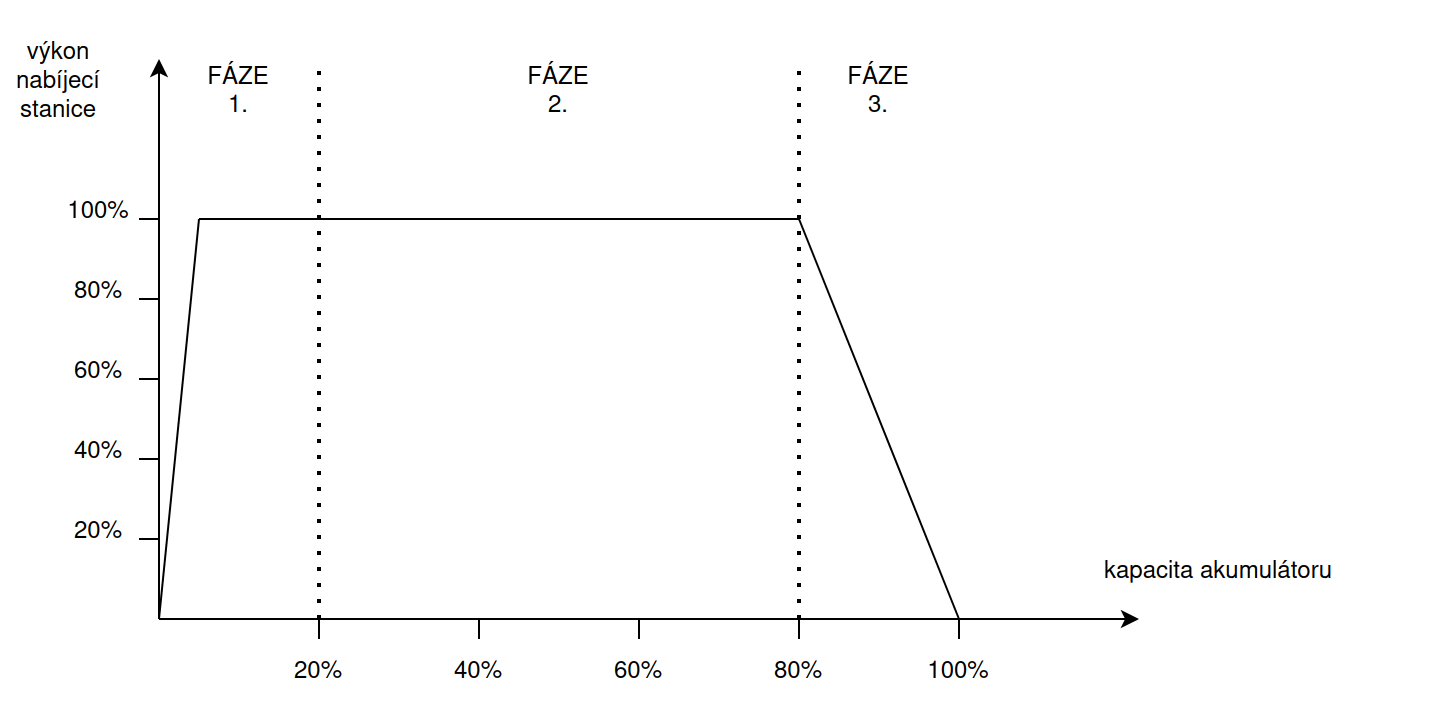
\includegraphics{ac-charging-efficency.eps}
    }
    \caption{Efektivita nabíjení pomocí střídavého proudu \cite{evbox_ac_dc}}
    \label{figure:ac-charging-efficency}
\end{figure}

\subsubsection{Nabíjení pomocí stejnosměrného proudu (DC)}
Křivka nabíjecího výkonu na obrázku \ref{figure:dc-charging-efficency} při využití stejnosměrného proudu se skládá ze tří fází.

V první fázi nabíjení dochází k postupnému zvyšování výkonu, protože akumulátor začíná nabíjení s nulovou úrovní nabití.
Nabíjecí stanice zajišťuje, aby proces probíhal bezpečně, což vyžaduje opatrné navyšování proudu. Výkon dosahuje svého
maxima při dosažení 20 \% kapacity baterie.

Ve druhé fázi výkon postupně klesá, a to z maximální hodnoty dosažené v první fázi na přibližně 70~\% maximálního výkonu. I přes tento pokles výkonu je tato fáze stále efektivní, protože většina kapacity baterie se nabíjí právě
v tomto rozmezí.

Jakmile baterie dosáhne přibližně 80 \% své kapacity, výkon začíná klesat. Tento proces je nezbytný pro ochranu baterie
před přehřátím nebo přetížením, což by mohlo vést ke snížení její životnosti. Posledních 20 \% nabíjení je tedy
pomalejší a méně efektivní. \cite{ivy_charge}

\begin{figure}[H]
    \centering
    \scalebox{0.25}{
        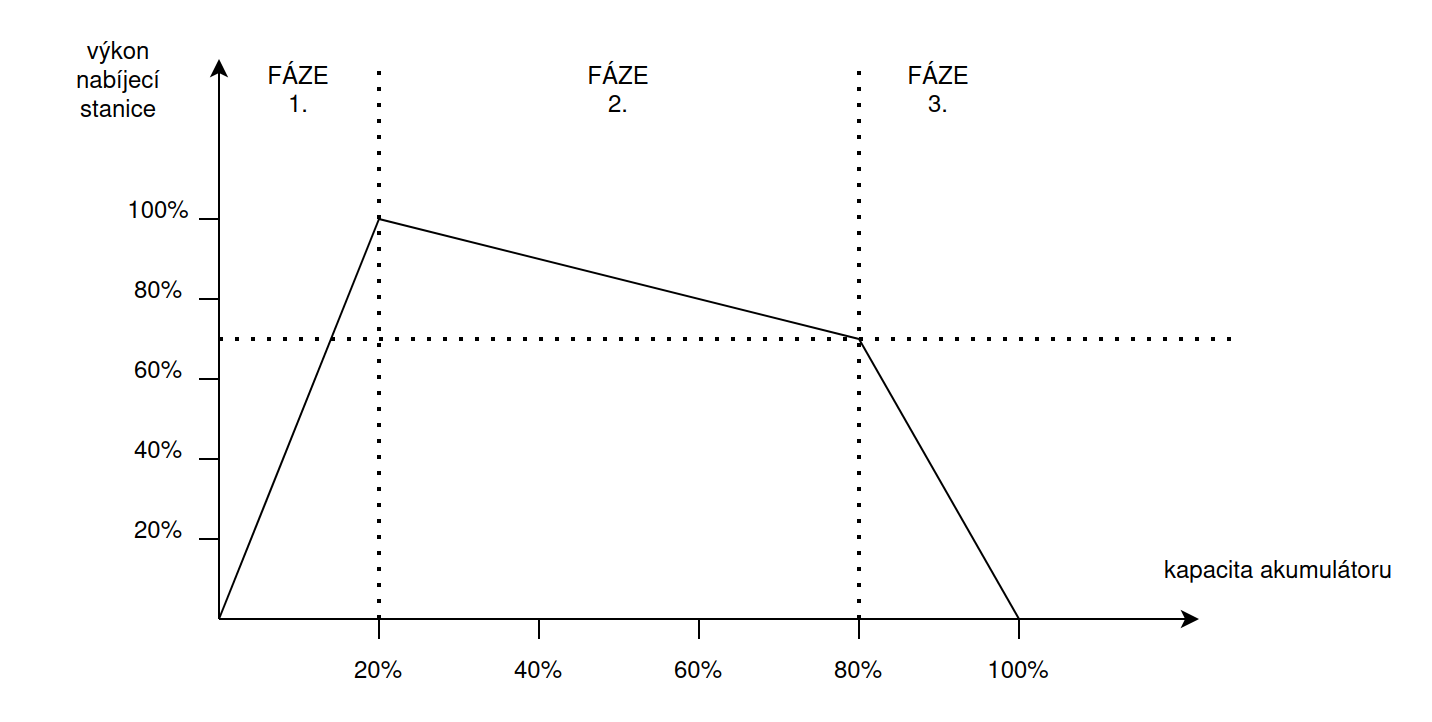
\includegraphics{dc-charging-efficency.eps}
    }
    \caption{Efektivita nabíjení pomocí stejnosměrného proudu \cite{evesco_dc_fast_charging}}
    \label{figure:dc-charging-efficency}
\end{figure}


\subsubsection{Výpočty průměrných nabíjecích výkonů nabíječek}
Pro výpočet průměrných nabíjecích výkonů uvedených v tabulce \ref{table:average-charging-power} byly využity křivky znázorňující nabíjecí průběhy AC a DC nabíjecích stanic, které jsou zobrazeny na obrázcích \ref{figure:ac-charging-efficency} a \ref{figure:dc-charging-efficency}. Nabíjení bylo rozděleno do tří fází na základě kapacity akumulátoru: \textit{0–20 \%}, \textit{20–80 \%} a \textit{80–100 \%}. Pro každou fázi byl průměrný výkon stanoven následujícím způsobem.\\

U AC nabíjení byl počáteční prudký nárůst výkonu v první fázi (\textit{0–20 \%}) zanedbán, protože se odehrál v rámci kapacity akumulátoru \textit{0–5 \%}, což bylo považováno za zanedbatelný interval. Tento interval byl opomenut také proto, že jen velmi malé množství vozidel dorazí k nabíjecí stanici s akumulátorem vybitým natolik, aby spadalo do tohoto rozsahu nabíjení. Proto byl výkon v první fázi považován za konstantní na úrovni 100 \% maximálního výkonu. Ve druhé fázi (\textit{20–80 \%}) byl výkon rovněž konstantní na úrovni 100 \%. Ve třetí fázi (\textit{80–100 \%}) výkon klesal lineárně z 100 \% na 0 \% maximální hodnoty, což dává průměrnou hodnotu 50 \% pro tento interval.\\

U DC nabíjení výkon v první fázi (\textit{0–20 \%}) lineárně roste z 0 \% na 100 \%, což odpovídá průměru 50 \% maximálního výkonu nabíjecí stanice. Ve druhé fázi (\textit{20–80 \%}) výkon lineárně klesal z 100 \% na 70 \% maximální hodnoty, což odpovídá průměrné hodnotě 85 \% pro tento interval, jak je patrné z grafu. Ve třetí fázi (\textit{80–100 \%}) dochází k postupnému poklesu výkonu z 70 \% na 0 \%, což odpovídá průměrnému výkonu 35 \% maximální hodnoty.\\

Procentuální hodnoty získané z analýzy průběhu nabíjení byly využity k výpočtu průměrného výkonu pro jednotlivé fáze. Pro každý interval nabíjení byl výkon vypočítán pomocí následujícího vzorce:

\[
P_{\text{průměr}} = P_{\text{max}} \cdot \frac{p_{\text{start}} + p_{\text{end}}}{2}
\]

kde:
\begin{itemize}
    \item \(P_{\text{průměr}}\) je průměrný výkon pro danou fázi,
    \item \(P_{\text{max}}\) je maximální výkon nabíjecí stanice,
    \item \(p_{\text{start}}\) je procentuální hodnota výkonu na začátku fáze (vyjádřená jako zlomek, např. \(p_{\text{start}} = 0.75\) pro 75 \%),
    \item \(p_{\text{end}}\) je procentuální hodnota výkonu na konci fáze (vyjádřená jako zlomek, např. \(p_{\text{end}} = 1.00\) pro 100 \%).\\
\end{itemize}

Například pro třetí fázi DC nabíjení (\textit{80–100 \%}) byl výkon stanoven následovně: \\

Maximální výkon nabíjecí stanice byl \(P_{\text{max}} = 50 \, \mathrm{kW}\), přičemž výkon v této fázi klesal lineárně z \(p_{\text{start}} = 0.70\) (70 \%) na \(p_{\text{end}} = 0.00\) (0 \%). Průměrný výkon této fáze lze tedy vypočítat takto:

\[
P_{\text{průměr}} = 50 \cdot \frac{0.70 + 0.00}{2} = 50 \cdot 0.35 = 17.5 \, \mathrm{kW}
\]

Podobným způsobem byly provedeny výpočty pro všechny fáze nabíjení jednotlivých nabíjecích stanic, přičemž výsledné hodnoty byly zaokrouhleny pro větší přehlednost.


\begin{table}[H]
    \centering 
    \vspace{0.5cm} % Space before table
    \begin{tabular}{|c|c|c|c|}
        \hline
        \textbf{} & \textbf{0 - 20 [\%]} & \textbf{20 - 80 [\%]} & \textbf{80 - 100 [\%]}\\
        \hline
        11 kWh AC  &  11 kWh  & 11 kWh & 5.5 kWh     \\
        \hline
        12 kWh AC  &  12 kWh  & 12 kWh & 6 kWh     \\
        \hline
        22 kWh AC  &  22 kWh  & 22 kWh & 11 kWh  \\
        \hline
        50 kWh DC  &  25 kWh  & 42.5 kWh & 17.5 kWh    \\
        \hline
        108 kWh DC &  54 kWh  & 91.8 kWh & 37.8 kWh \\
        \hline
        150 kWh DC &  75 kWh  & 127.5 kWh & 52.5 kWh \\
        \hline
    \end{tabular}
    \caption{Průměrný nabíjecí výkon pro jednotlivé fáze nabíjení}
    \label{table:average-charging-power}
    \vspace{0.5cm} % Space after table
\end{table}


\subsubsection{Výpočty průměrných dob potřebných k nabití baterie}

Pro výpočet průměrné doby potřebné k nabití baterie byly využity hodnoty průměrného nabíjecího výkonu uvedené v tabulce \ref{table:average-charging-power} a průměrná kapacita baterie \(71.6 \, \mathrm{kWh}\), o níž se pojednává v podkapitole \ref{batteries}. Výpočty byly provedeny pro každou fázi nabíjení (\textit{0–20 \%}, \textit{20–80 \%}, \textit{80–100 \%}) zvlášť pomocí následujícího vzorce:

\[
t_{\text{nabíjení}} = \frac{C_{\text{baterie}}}{P_{\text{průměr}}} \cdot k_{\text{fáze}}
\]

kde:
\begin{itemize}
    \item \(t_{\text{nabíjení}}\) je maximalní doba nabíjení v dané fázi [h],
    \item \(C_{\text{baterie}}\) je průměrná kapacita baterie elektromobilů (\(71.6 \, \mathrm{kWh}\)),
    \item \(P_{\text{průměr}}\) je průměrný nabíjecí výkon v dané fázi (viz tabulka \ref{table:average-charging-power}) [kW],
    \item \(k_{\text{fáze}}\) je podíl kapacity baterie nabíjený v dané fázi (např. \(0.2\) pro fázi \textit{0–20 \%}).\\
\end{itemize}

Například pro fázi \textit{20–80 \%} (odpovídající \(k_{\text{fáze}} = 0.6\)) a DC nabíjecí stanici s maximálním výkonem \(50 \, \mathrm{kWh}\) lze výpočet provést následovně:

\[
t_{\text{nabíjení}} = \frac{71.6}{42.5} \cdot 0.6 = 1.01 \, \mathrm{h}
\]

Podobným způsobem byly vypočteny časy nabíjení pro všechny fáze a typy nabíjecích stanic. Výsledné hodnoty jsou uvedeny v tabulce \ref{table:charging-time-consumption}.


\begin{table}[H]
    \centering 
    \vspace{0.5cm} % Space before table
    \begin{tabular}{|c|c|c|c|}
        \hline
        \textbf{} & \textbf{0 - 20 [\%]} & \textbf{20 - 80 [\%]} & \textbf{80 - 100 [\%]}\\
        \hline
        11 kW AC  &  0 -- 1.30 h  & 0 -- 3.90 h & 0 -- 2.60 h  \\
        \hline
        12 kW AC  &  0 -- 1.19 h  & 0 -- 3.58 h & 0 -- 2.38 h  \\
        \hline
        22 kW AC  &  0 -- 0.65 h  & 0 -- 1.95 h & 0 -- 1.30 h  \\
        \hline
        50 kW DC  &  0 -- 0.57 h & 0 -- 1.01 h & 0 -- 0.82 h  \\
        \hline
        108 kW DC &  0 -- 0.26 h  & 0 -- 0.47 h & 0 -- 0.38 h  \\
        \hline
        150 kW DC &  0 -- 0.19 h  & 0 -- 0.34 h & 0 -- 0.27 h  \\
        \hline
    \end{tabular}
    \caption{Čas potřebný k nabití baterie v jednotlivých fázích stanic}
    \label{table:charging-time-consumption}
    \vspace{0.5cm} % Space after table
\end{table}


\subsubsection{Petriho síť elektromobility v Brně}

Na začátku je nutné simulovat generování automobilů v určitém časovém intervalu. V našem modelu je tento proces reprezentován exponenciálním rozložením s parametrem \(\lambda\). Protože jsme chtěli simulovat celodenní (24 hodin), denní (14 hodin) i noční režim (10 hodin), v návrhu Petriho sítě parametr \(\lambda\) konkrétně nedefinujeme. Když se elektromobil vygeneruje, zařadí se do fronty, která reprezentuje elektromobily v Brně, jež se chtějí nabít. 

Každý elektromobil je následně zařazen do specifické fronty podle aktuálního stavu baterie. Největší část elektromobilů (80 \%) má stav baterie v rozmezí 20–80 \% a potřebuje se dobít. Pravděpodobnost, že elektromobil přijede s kapacitou baterie pod 20 \% nebo nad 80 \%, je shodně 10 \%. Při volbě těchto údajů jsme vycházeli ze skutečnosti, že většina lidí se snaží udržovat své baterie v rozmezí 20–80~\%, jak již bylo zmíněno v podkapitole \ref{batteries}. Po zařazení do fronty si elektromobil vybírá výkon nabíječky, kterou chce použít. Pravděpodobnost výběru konkrétního typu nabíječky je vypočítána na základě poměru počtu daného typu nabíječek k celkovému počtu nabíječek. 

Po výběru nabíječky elektromobil přejde do stavu čekání ve frontě na nabíječku s daným výkonem. Přechod do stavu nabíjení je možný pouze v případě, že sklad nabíječek daného výkonu má volnou alespoň jednu nabíječku. Jakmile je nabíječka volná, elektromobil si ji zabere a začne proces nabíjení (během této fáze čeká po dobu simulovanou rovnoměrným rozložením). Rozsahy pro rovnoměrné rozložení nabíjecí doby jsou uvedeny v tabulce \ref{table:charging-time-consumption}.


Po dokončení nabíjení může elektromobil:
\begin{itemize}
    \item přejít do další fáze nabíjení (v případě, že přešel z první fáze, kdy měl kapacitu baterie 0–20 \%, na druhou fázi s kapacitou 20–80 \%),
    \item nebo dokončit nabíjení, uvolnit nabíječku a opustit systém.
\end{itemize}

Při přechodu z první fáze nabíjení (0 -- 20 \%) do druhé fáze (20 -- 80 \%) je důležité poznamenat, že elektromobil už nemusí znovu čekat ve frontě na nabíječku, protože ji má stále obsazenou. Rovnou tedy přechází do fáze nabíjení z 20 na 80 \% kapacity baterie. Po této fázi uvolní nabíječku a systém opustí.

Třetí fáze nabíjení, tedy z 80 na 100 \% kapacity baterie, simuluje elektromobily, které do systému přijedou s kapacitou baterie vyšší než 80 \% a chtějí se nabít na plnou kapacitu. Tyto elektromobily postupují stejným způsobem jako ostatní, avšak jejich proces začíná přímo touto třetí fází.


\begin{figure}[H]
    \centering
    \scalebox{0.135}{
        \includegraphics{ims-petri-net.eps}
    }
    \caption{Petriho síť elektromobility v Brně}
    \label{figure:ims-petri-net}
\end{figure}

\section{Simulace elektromobility}

\subsection{Vstupy a výstupy programu}

Program byl implementován na základě návrhu Petriho sítí (viz obrázek \ref{figure:ims-petri-net}). Tento model slouží k simulaci nabíjení elektromobilů v rámci města s různými režimy provozu a nabíjecími stanicemi.

\subsubsection{Vstupy programu}

Program se spouští s následujícím základním formátem:

\begin{verbatim}
./sim [d|n|24h] [-tc počet_aut] [-p procento] [-ac11 počet] [-ac12 počet]
[-ac22 počet] [-dc50 počet] [-dc108 počet] [-dc150 počet] [-h]
\end{verbatim}

Popis jednotlivých parametrů:
\begin{itemize}
    \item \texttt{[d|n|24h]}: Režim simulace.
    \begin{itemize}
        \item \texttt{d}: Denní režim (od 7:00 do 21:00, tj. 14 hodin).
        \item \texttt{n}: Noční režim (od 21:00 do 7:00, tj. 10 hodin).
        \item \texttt{24h}: Simulace celého dne (24 hodin).
    \end{itemize}
    \item \texttt{-tc počet\_aut}: Počet elektromobilů ve městě.
    \item \texttt{-p procento}: Procento elektromobilů ve městě, která se v daný den budou chtít nabít. Na základě tohoto procenta se vypočítává parametr \(\lambda\) pro generování počtu aut (např. hodnota \texttt{0.25} znamená 25 \% elektromobilů z celkového počtu elektromobilů ve městě).
    \item \texttt{-ac11 počet}, \texttt{-ac12 počet}, \texttt{-ac22 počet}, \texttt{-dc50 počet}, \texttt{-dc108 počet}, \texttt{-dc150 počet}: Počet nabíjecích bodů pro stanice s příslušným výkonem (např. AC 11 kW, DC 50 kW apod.).
    \item \texttt{-h}: Zobrazení nápovědy a možností spuštění programu.
\end{itemize}


\subsubsection{Výchozí hodnoty}
V programu jsou výchozí hodnoty parametrů nastaveny na aktuální situaci ve městě Brno:
\begin{itemize}

    \item \texttt{-tc}: Počet elektromobilů je nastaven na hodnotu 1700, což odpovídá odhadu aktuálního počtu elektromobilů v Brně. Tento odhad byl získán analýzou dat poskytnutých nemenovanou společností.
    \item \texttt{-p}: Procento elektromobilů, která se chtějí nabít v danou periodu, bylo vypočítáno na základě analýzy datového souboru od nemenované společnosti. Pro denní režim (\texttt{d}) činí toto procento 17.7 \%, zatímco pro noční režim (\texttt{n}) odpovídá jedné desetině této hodnoty, tj. 1.77 \%.
    \item Počet jednotlivých nabíjecích stanic (\texttt{-ac11}, \texttt{-ac12}, \texttt{-ac22}, \texttt{-dc50}, \texttt{-dc108}, \texttt{-dc150}) byl určen z dat a je podrobněji popsán v podkapitole \ref{dataset-processing}.
\end{itemize}

\subsubsection{Výstupy programu}

Výstupy programu jsou zobrazovány v terminálu. Jedná se o následující údaje:
\begin{itemize}
    \item Počet generovaných automobilů ve zvoleném režimu simulace (denní, noční, 24 hodin).
    \item Počet automobilů, která zahájila proces nabíjení.
    \item Počet automobilů, která dokončila nabíjení a opustila systém.
    \item Průměrná doba potřebná k úplnému nabití baterie (od 0 \% do 100 \% kapacity).
    \item Statistiky jednotlivých skladů nabíjecích stanic, včetně využití.
    \item Statistiky čekacích dob ve frontách u jednotlivých nabíjecích stanic.
    \item Histogram znázorňující doby, po které se elektromobily nacházely v systému (od vstupu do systému po jeho opuštění).
\end{itemize}

V adresáři \texttt{output} jsou umístěny ukázkové výstupní textové soubory, jejichž názvy odpovídají parametrům zadaným při spuštění programu. Každý soubor obsahuje informace o statistikách skladů a histogramu.

Tyto výstupy umožňují analyzovat efektivitu nabíjecí infrastruktury, její vytíženost a čekací doby, což může být využito jako základ pro zlepšení efektivity provozu.

\subsection{Momentální stav elektromobility v Brně}
Program byl spuštěn s výchozími hodnotami, které definují aktuální stav elektromobility v Brně. Simulace byla provedena pro tři režimy: denní (\texttt{d}), noční (\texttt{n}) a celodenní (\texttt{24h}). 

Ze simulace bylo zjištěno, že nabíjecí stanice bez problémů pokrývají aktuální potřeby elektromobility v Brně, přičemž ve žádném z režimů simulace nedocházelo k tvorbě front ani přetížení infrastruktury. Tato zjištění potvrzují, že současná nabíjecí infrastruktura je dostatečně navržena pro pokrytí potřeb elektromobilů za výchozích podmínek simulace.

\paragraph{Výstup programu pro momentální stav\\\\}

Na základě simulace denního režimu (\texttt{d}), nočního režimu (\texttt{n}) a celodenního režimu (\texttt{24h}) byly získány následující výsledky:

\paragraph{Denní režim (\texttt{d}):} 
Denní režim, který pokrývá období od 7:00 do 21:00 (celkem 14 hodin), simuloval celkem 281 elektromobilů. Všechna vozidla zahájila nabíjení, přičemž 260 z nich proces úspěšně dokončilo a opustilo systém. Průměrná doba nabíjení z úplného vybití na plnou kapacitu byla 100,475 minut.

Podle histogramu času stráveného v systému se minimální doba pohybovala okolo 0,07 minuty a maximální dosáhla 188,17 minut. Průměrná doba činila 48,19 minut se směrodatnou odchylkou 38,31 minut. Největší podíl vozidel (30,77 \%) strávil v systému méně než 20 minut, zatímco přibližně 68 \% vozidel opustilo systém do 60 minut. Dlouhé časy nad 140 minut byly spíše výjimečné a tvořily méně než 3 \% případů. Tyto výsledky naznačují, že nabíjecí infrastruktura během denního režimu dokáže většinu vozidel obsloužit bez výrazného zpoždění.

\paragraph{Noční režim (\texttt{n}):}
V nočním režimu, který probíhá od 21:00 do 7:00 (celkem 10 hodin), simulace generovala 28 elektromobilů. Všechna tato vozidla zahájila nabíjení a 27 z nich nabíjení úspěšně dokončilo. Průměrná doba nabíjení byla delší než v denním režimu a dosáhla hodnoty 125,856 minut.

Podle histogramu se minimální doba strávená v systému pohybovala na 0,31 minutách, zatímco maximální činila 143,04 minut. Průměrná doba strávená v systému byla 62,55 minut, což je vyšší hodnota než v denním režimu. Největší podíl vozidel (25,93 \%) opustil systém v rozmezí 40 až 60 minut, přičemž dlouhé časy nad 140 minut byly výjimečné.

Celkově je zřejmé, že v nočním režimu je vytížení nabíjecí infrastruktury výrazně nižší než ve dne. Méně vozidel znamená plynulejší provoz a žádné fronty, což umožňuje efektivní obsloužení všech elektromobilů. Tento stav ukazuje, že noční režim není hlavním zdrojem zátěže pro nabíjecí infrastrukturu.


\paragraph{Celodenní režim (\texttt{24h}):}
Celodenní režim, zahrnující 24 hodin, simuloval celkem 310 elektromobilů. Všechna vozidla zahájila nabíjení, přičemž 307 z nich dokončilo proces a opustilo systém. Průměrná doba nabíjení dosáhla hodnoty 108,203 minut.

Histogram celkového času v systému ukazuje minimální dobu 0,07 minut a maximální 229,76 minut. Průměrná doba byla 53,65 minut, což je mezi hodnotami zjištěnými v denním (48,19 minut) a nočním režimu (62,55 minut). Největší podíl vozidel (27,04 \%) strávil v systému méně než 20 minut, zatímco dlouhé časy nad 140 minut byly opět spíše výjimečné. Tyto výsledky potvrzují schopnost infrastruktury zvládnout nabíjení většiny vozidel s minimálním zpožděním.

\paragraph{} 
Celkové výsledky simulace naznačují, že současná nabíjecí infrastruktura v Brně je schopná efektivně pokrýt poptávku elektromobilů. Vysoký počet dokončených nabíjení a relativně nízké průměrné časy v systému potvrzují, že infrastruktura je dobře přizpůsobena aktuálnímu počtu vozidel ve městě.

\subsection{Stav elektromobility v Brně v roce 2030}

S rostoucím počtem elektromobilů, který se očekává do roku 2030, je důležité pochopit, jak tento nárůst ovlivní stávající nabíjecí infrastrukturu v Brně. Počet elektromobilů by měl výrazně vzrůst, což klade nové nároky na kapacitu a dostupnost nabíjecích stanic. Očekává se, že rozšiřování nabíjecích bodů, delší dojezdy na jedno nabití a rychlejší nabíjení umožní širší přijetí elektromobility mezi uživateli. \cite{electromobiles_in_future}

Hlavním cílem tohoto experimentu je zjistit, jak zvýšený počet elektromobilů ovlivní čekací doby, vytíženost nabíjecích stanic a celkovou efektivitu nabíjecí infrastruktury. V rámci simulace jsme proto zohlednili různé scénáře, které počítají s různými počty a výkony nabíjecích bodů.

\subsubsection{Nárůst elektromobilů}
Abychom mohli simulovat situaci v roce 2030, bylo potřeba odhadnout přibližný počet elektromobilů v Brně. Na základě informací z článku \cite{ev_growth} odhadujeme, že počet elektromobilů by na konci roku 2030 mohl dosáhnout přibližně 20 tisíc.

Tento odhad nám poskytuje výchozí bod pro experimenty zaměřené na analýzu dopadů zvýšeného počtu elektromobilů na nabíjecí infrastrukturu ve městě. Simulace nám umožní zjistit, jak se infrastruktura vyrovná s větší zátěží a jak by ji bylo možné přizpůsobit rostoucí poptávce.

\subsubsection{Simulace nabíjení při stávající infrastruktuře}
Pro první část simulace jsme ponechali počty nabíjecích stanic nezměněné, aby odpovídaly současnému stavu infrastruktury v Brně. Jedinou změnou byl zvýšený počet elektromobilů, který jsme nastavili na 20 000 podle předchozího odhadu. Kromě toho jsme zvýšili podíl elektromobilů, která se chtějí během jednoho dne nabíjet, na 25 \%. Tento vyšší podíl odráží předpoklad, že v budoucnosti budou elektromobily používány častěji, což povede k větší zátěži na nabíjecí infrastrukturu.

Cílem této simulace bylo zjistit, zda stávající infrastruktura dokáže zvládnout zvýšený počet vozidel, a identifikovat klíčové problémy, jako jsou fronty u nabíjecích stanic nebo prodloužené čekací doby. Tato analýza poskytuje důležitý základ pro návrh efektivnějšího řešení do budoucna.


\paragraph{Výstup programu\\\\}
Na základě simulace denního režimu (\texttt{d}), nočního režimu (\texttt{n}) a celodenního režimu (\texttt{24h}) jsme získali následující výstupy:

\paragraph{Denní režim (\texttt{d}):} 
V rámci 14hodinového denního režimu, který probíhá od 7:00 do 21:00, bylo simulováno celkem 5 133 elektromobilů. Z tohoto počtu se 4 373 vozidel, tedy 85 \%, připojilo k nabíjení. Plně nabít a opustit systém však zvládlo pouze 4 110 elektromobilů, což odpovídá 80 \% generovaných vozidel. Tato čísla naznačují, že současná nabíjecí infrastruktura má problémy s pokrytím zvýšené poptávky.

Průměrná doba nabíjení zůstala na úrovni 102,45 minut, což je srovnatelné s předchozími výsledky. Přesto 15 \% elektromobilů nabíjení vůbec nezahájilo a dalších 5 \% ho nedokončilo, což ukazuje na obtíže systému zvládnout větší počet elektromobilů.

Podrobnější analýza odhalila výrazné fronty u pomalejších AC nabíječek:
\begin{itemize}
    \item \textbf{11 kW nabíječky}: Průměrná fronta činila 23 vozidel, tedy zhruba 4 vozidla na jednu nabíječku.
    \item \textbf{12 kW nabíječky}: Fronty byly ještě delší, v průměru 87 vozidel, což odpovídá více než 4 vozidlům na jednu nabíječku.
    \item \textbf{22 kW nabíječky}: Průměrná fronta zde dosahovala 251 vozidel. Při kapacitě 197 nabíječek to odpovídá zhruba 1,27 vozidla na jednu nabíječku.
\end{itemize}

Naopak u rychlejších \textbf{DC nabíječek} (50 kW, 108 kW, 150 kW) se fronty vůbec nevytvářely. Statistika ukázala:
\begin{itemize}
    \item \textbf{50 kW nabíječky}: Průměrně bylo využíváno 36 z 54 dostupných bodů.
    \item \textbf{108 kW nabíječky}: Průměrné využití bylo 2,6 bodu z celkových 11.
    \item \textbf{150 kW nabíječky}: V průměru bylo obsazeno 3,6 bodu z 17.
\end{itemize}

Tato data potvrzují, že \textbf{DC nabíječky} jsou mnohem efektivnější a umožňují rychlé nabíjení, zatímco \textbf{AC nabíječky} omezují plynulost systému a způsobují značné fronty.

Podle histogramu byla \textbf{průměrná doba v systému} 95 minut, což je 1 hodina a 35 minut, se směrodatnou odchylkou 78 minut. Maximální doba v systému byla téměř 9 hodin, což by pro uživatele znamenalo neúnosné čekání. 

Z výsledků je zřejmé, že současná infrastruktura má zásadní nedostatky, zejména u AC nabíječek. K zajištění plynulého provozu by bylo nutné rozšířit kapacitu nebo přejít na výkonnější DC nabíječky.

\paragraph{Noční režim (\texttt{n}):} 
Během nočního režimu, který trvá 10 hodin (od 21:00 do 7:00), bylo simulováno 464 elektromobilů. Všechna vozidla zahájila nabíjení, z nichž 425 úspěšně dokončilo proces a opustilo systém. 

Detailní analýza ukázala, že během nočního režimu se netvořily žádné fronty u nabíjecích stanic. Průměrná doba, kterou vozidla strávila v systému, byla 51 minut se směrodatnou odchylkou 38 minut. Tato čísla naznačují, že infrastruktura byla během nočního režimu dostatečně efektivní a umožnila plynulý provoz bez zpoždění.


\paragraph{Celodenní režim (\texttt{24h}):} 
V celodenním režimu bylo vygenerováno celkem 5 638 elektromobilů, z nichž 5 505 zahájilo nabíjení. To odpovídá 97 \% všech vygenerovaných vozidel, což je výrazné zlepšení oproti dennímu režimu, kde se k nabíjení připojilo pouze 85 \% aut. Hlavním důvodem tohoto rozdílu je skutečnost, že vozidla generovaná během dne mohla pokračovat v nabíjení i po 21. hodině. Celkově 5 442 vozidel úspěšně dokončilo nabíjení a opustilo systém, což představuje 96 \% všech generovaných elektromobilů. Tento výsledek lze považovat za dobrý, ale v reálném světě by uživatelé pravděpodobně nechtěli nabíjet své vozy na veřejných stanicích dlouho do noci.

Fronty se během celodenního režimu tvořily pouze u AC nabíječek. Průměrná délka front dosahovala přibližně 3,5 vozidla na jednu AC nabíječku, což je sice méně než v denním režimu, ale stále to představuje významný problém. Navíc byla průměrná doba, kterou vozidla strávila v systému, 122 minut se směrodatnou odchylkou 120 minut. To znamená, že někteří uživatelé čekali na dokončení nabíjení výrazně déle.

Výsledky naznačují, že pokud se má zvládnout rostoucí počet elektromobilů, bude nutné zvýšit počet DC nabíjecích bodů. Tyto stanice nabízejí rychlejší nabíjení a mohou výrazně zlepšit plynulost celé infrastruktury.


\subsubsection{Simulace nabíjení při rozšířené infrastruktuře}

Na základě informací z článku \cite{ev_growth}, který uvádí, že město Brno plánuje do roku 2030 vybudovat síť 1 000 nabíjecích bodů, jsme se rozhodli analyzovat, jak by takové rozšíření infrastruktury ovlivnilo efektivitu nabíjení elektromobilů v nejvytíženějším denním režimu, tedy od 7:00 do 21:00. Provedli jsme dva experimenty, každý s odlišným rozšířením nabíjecích stanic.


\paragraph{Experiment 1: Zvýšení počtu AC nabíječek\\\\}
V tomto experimentu jsme se zaměřili na navýšení počtu \textbf{AC nabíječek} na celkových 1 000 bodů. Pro 11 kW a 12 kW nabíječky bylo přidáno po 300 bodů a pro 22 kW nabíječky 400 bodů (\texttt{./sim d -tc 20000 -p 0.25 -ac11 300 -ac12 300 -ac22 400}). Cílem bylo zjistit, jak by toto navýšení ovlivnilo fungování systému a zvládání poptávky v denním režimu (od 7:00 do 21:00).

Simulace ukázala, že během dne bylo vygenerováno 5 039 elektromobilů a všechna tato vozidla se připojila k nabíjecím stanicím. Nabít a opustit systém se ale podařilo pouze 4 490 vozidlům, což odpovídá 89~\% všech generovaných aut.

Průměrná doba nabíjení dosáhla 168 minut, což je téměř o hodinu více než ve scénáři se stávající infrastrukturou, kde bylo nabíjení zvládnuto za průměrných 102 minut. Tento výsledek naznačuje, že i při navýšení počtu AC nabíječek systém nedokázal eliminovat zdržení způsobená pomalým nabíjením na těchto typech stanic.

Průměrná doba v systému byla 83 minut s odchylkou 60 minut, což naznačuje, že některé elektromobily zůstávaly v systému mnohem déle. Minimální doba byla 0,03 minuty, zatímco maximální dosáhla téměř 5 hodin. Přibližně 6~\% vozidel strávilo v systému více než 3 hodiny, což může být pro uživatele nepřijatelné.

Na druhou stranu, navýšení počtu AC nabíječek zajistilo, že se během simulace netvořily žádné fronty, což znamená, že z hlediska dostupnosti bylo stanic dostatek. Navzdory tomu pomalé nabíjení způsobovalo, že systém nebyl dostatečně efektivní pro zvládnutí vysokého počtu elektromobilů. Výsledky ukazují, že pouhé navýšení kapacity AC nabíječek nestačí a že by mělo být doplněno rozšířením rychlejších DC nabíječek.


\paragraph{Experiment 2: Zvýšení počtu AC a DC nabíječek\\\\}
Ve druhém experimentu jsme kombinovali navýšení počtu \textbf{AC i DC nabíječek}, přičemž celkový počet bodů (AC a DC dohromady) byl opět 1 000. V tomto scénáři byly parametry nastaveny na 200 bodů pro 11kW a 12kW stanice, 250 bodů pro 22kW stanice, 150 bodů pro DC 50kW stanice a 100 bodů pro DC 108kW a 150kW stanice (\texttt{./sim d -tc 20000 -p 0.25 -ac11 200 -ac12 200 -ac22 250 -dc50 150 -dc108 100 -dc150 100}). Tento experiment zkoumal, zda kombinace rychlejších DC a pomalejších AC nabíječek dokáže zlepšit dostupnost infrastruktury ve srovnání s pouhým zvýšením počtu AC nabíječek.

Program simuloval celkem 5 059 elektromobilů, přičemž všechna vozidla zahájila proces nabíjení. Systém úspěšně opustilo plně nabito 4 666 vozidel, což odpovídá 92 \% všech generovaných elektromobilů. Průměrná doba potřebná k dokončení nabíjení činila 127 minut, což je o 29 minut méně než v prvním experimentu, kde bylo zvýšeno pouze množství AC nabíječek. Tento výsledek ukazuje, že kombinace rychlejších DC nabíječek a pomalejších AC nabíječek umožňuje zlepšit efektivitu nabíjení.

Podrobný výstup ukazuje, že se v průběhu simulace nevytvořily žádné fronty u nabíjecích stanic. To naznačuje, že dostupnost nabíjecích bodů byla zcela dostatečná. V porovnání s prvním experimentem, kde se rovněž nevytvářely fronty, je klíčovým rozdílem právě průměrná doba nabíjení, která byla v tomto experimentu výrazně kratší.

Histogram ukazuje, že většina vozidel (přes 31 \%) opustila systém za méně než 20 minut, což je výrazné zlepšení oproti prvnímu experimentu. Průměrná doba strávená v systému činila 62 minut se směrodatnou odchylkou 59 minut. Tento výsledek je o 15 minut lepší než v prvním experimentu.

Z analýzy je zřejmé, že DC nabíječky byly v průměru méně vytížené než AC nabíječky. Například DC 50kW stanice využívaly průměrně 30 ze 150 dostupných bodů, zatímco 11kW a 12kW AC stanice byly v průměru využity na 127 a 114 bodů z celkových 200. Tato data potvrzují, že rychlejší DC nabíječky výrazně snižují zatížení systému a zlepšují plynulost nabíjení.

\section{Závěr}
Tento projekt se zaměřil na zkoumání současné a budoucí situace elektromobility v Brně pomocí simulací nabíjecí infrastruktury. Cílem bylo zjistit, jak dobře si stávající systém poradí s rostoucím počtem elektromobilů a jak by mohla rozšířená infrastruktura zlepšit dostupnost a rychlost nabíjení.

Simulace ukázaly, že aktuální stav nabíjecí sítě v Brně je dostatečný pro současný počet elektromobilů. Systém zvládá poptávku bez větších problémů -- nevznikají dlouhé fronty a většina vozidel je nabita v rozumném čase. Nicméně při předpokládaném nárůstu počtu elektromobilů na 20 tisíc do roku 2030 se ukázaly zásadní slabiny. Hlavním problémem jsou pomalejší AC nabíječky, které nedokážou zvládnout vyšší počet vozidel a způsobují zdržení a fronty.

Pro zlepšení situace byly provedeny dva experimenty s rozšířením nabíjecí sítě, přičemž počet nabíjecích bodů byl zvolen na základě článku \cite{ev_growth}, který uvádí, že Teplárny Brno plánují do roku 2030 vybudovat 1 000 nabíjecích bodů. Experimenty se zaměřily na dvě varianty rozšíření infrastruktury:

\begin{description}
    \item[\textbf{Zvýšení počtu AC nabíječek}] V prvním experimentu byl počet AC nabíjecích bodů navýšen na 1 000. Toto rozšíření eliminovalo fronty, což ukazuje na dostatečnou kapacitu stanic. Průměrná doba strávená v systému však byla 82,88 minut s odchylkou 60,19 minut, což je pro uživatele stále příliš dlouhé a nevyhovující.
    \item[\textbf{Kombinace AC a DC nabíječek}] Druhý experiment kombinoval navýšení počtu pomalejších AC nabíječek a rychlejších DC nabíječek, přičemž celkový počet bodů zůstal na 1 000. Tato kombinace přinesla výrazně lepší výsledky. Průměrná doba strávená v systému byla 61,83 minut s odchylkou 58,57 minut. DC nabíječky se ukázaly jako klíčové pro efektivní zvládnutí vyšší poptávky a významně zlepšily plynulost celého systému. Přibližně 70~\% elektromobilů strávilo v systému méně než 80 minut, což představuje značné zlepšení oproti prvnímu experimentu.
\end{description}

Z výsledků experimentů vyplývá, že samotné navýšení počtu AC nabíječek nestačí. Rychlejší DC nabíječky výrazně snižují dobu nabíjení a zvyšují efektivitu systému, což je nezbytné pro zvládnutí vyššího počtu elektromobilů v budoucnosti. Kombinace AC a DC nabíječek se ukazuje jako nejefektivnější způsob, jak zajistit plynulé a rychlé nabíjení a zároveň minimalizovat čekací doby.

Brno by se mělo zaměřit na rozšíření nabíjecí infrastruktury, která kombinuje oba typy nabíječek. Taková síť umožní městu zvládnout přechod na ekologičtější a udržitelnější dopravu. Výsledky projektu jasně ukazují, že investice do rozšíření infrastruktury s důrazem na DC nabíječky budou nezbytné pro přípravu na budoucí požadavky elektromobility a pro zajištění komfortu uživatelů.

\newpage
\bibliographystyle{unsrt}
\bibliography{resources}
\label{sec:zdroje}

\end{document}